\pdfoutput=1

\documentclass{l4proj}

%
% put any packages here
%
\usepackage{float}
\usepackage{enumitem}
\usepackage{longtable}
\usepackage{listings}
\usepackage{hyperref}
\usepackage{subfiles}
\usepackage{color}
\usepackage{graphicx}


\newcommand{\nc}[1]{\textcolor{magenta}{(\textbf{NC:} #1)}}
\newcommand{\gac}[1]{\textcolor{cyan}{(\textbf{GAC:} #1)}}
\newcommand{\pwt}[1]{\textcolor{blue}{(\textbf{PWT:} #1)}}

\graphicspath{{images}{../images/}}

\begin{document}
\title{Evaluating the Scalability of ROS in Multi-Robot Systems}
\author{Isaac Jordan}
\date{\today}
\maketitle

\begin{abstract}
Robots, distributed systems, and middleware.
\end{abstract}

\educationalconsent
%
%NOTE: if you include the educationalconsent (above) and your project is graded an A then
%      it may be entered in the CS Hall of Fame
%
\tableofcontents
%==============================================================================

\pagebreak
\pagenumbering{arabic}

\subfile{sections/introduction}

%\vspace{-7mm}
%\begin{figure}
%\centering
%\includegraphics[height=9.2cm,width=13.2cm]{uroboros.pdf}
%\vspace{-30mm}
%\caption{An alternative hierarchy of the algorithms.}
%\label{uroborus}
%\end{figure}

\chapter{Background}
\label{background-chapter}

\subfile{sections/background-part1}

\subfile{sections/background-part2-middleware-overview}

\subfile{sections/background-part3-middleware-discussion}

\subfile{sections/background-part4}

\chapter{Communication Scalability}
\label{communication-chapter}

Multi-robot systems are types of distributed systems. The main concern in moving from a single-host distributed system to a multi-host distributed system is the introduction of more complex communication network. As the overall system is trying to complete a task, the individual nodes in the network must communicate in order to share things like the status of the node (CPU load, disk usage, etc), progress through the current task, and results of a task. The exact nature and direction of this communication is dependent on the architecture of the distributed system.

In ROS, the Master node monitors the progress and status of the other nodes, but does not involve itself in the application logic of the system, meaning that it does not process or handle the results of nodes. This is handled in a peer-to-peer (P2P) fashion dictated by the application developer - each node is responsible for choosing what information to request from other nodes, and what information to emit from itself using the Publisher/Subscriber model described in Section \ref{background-ros}. The consequence of this architecture is that overall system performance can be dramatically affected by the communication performance between nodes.

The communication experiments look in to the scalability of communication in ROS. How well does it handle having to send high frequency work-loads of varying sizes.

In order to systematically evaluate how ROS' communication scales, we first aim to understand the aspects of the system that are of greatest importance to performance - both in terms of latency of messages, and total throughput of communication. Section \ref{communication-scoping-experiments} aims to analyse the performance bottlenecks of a simple multi-robot system when sending very controlled and artificial data. Section \ref{communication-real-data} will then aim to validate the results of Section \ref{communication-scoping-experiments} using realistic (previously recorded) data streams, with the goal that these conclusions wil then be directly applicable to real ROS multi-robot systems.

\section{Scoping Experiments}
\label{communication-scoping-experiments}



Scoping experiments were quick experiments using dummy data. Designed to identify useful areas to explore in more detail in realistic experiments later.

\subfile{sections/experiment1}

\subfile{sections/experiment2}

\subfile{sections/experiment3}

\subfile{sections/experiment4}

\section{Realistic Data Experiments}
\label{communication-real-data}

Previous experiments were presented as scoping experiments. These were designed to systematically understand which variables were of concern when running tests on ROS's communication performance. However, it was not certain that these prior conclusions would translate well to using ROS in a realistic scenario. Throughout the scoping experiments, the same message of `hello world' was used as dummy data.

In order to verify the conclusions were correct, samples of realistic data was explored. Two likely data types were settled on, `sensor data' and `video data'.

Sensor data is the type of data likely the come from a physical sensor on the robot. This data is characterised by small message sizes, such as 4KB.

Video data used was a 30Hz (30 frames-per-second) RGB video stream, with a resolution of 640 x 480 pixels. This message stream was measured to use 9.25MB/s of bandwidth, implying a message size of 308KB.

Both data sets were acquired from the MIT Stata Center dataset \cite{mit-stata-center-dataset}. This dataset contains both sensor feeds (such as from a laser sensor), and video feeds (from a Kinect RGB + depth camera). These data sets are very large (20 - 50GB) which would require modification to the test system (Raspberry Pi 3’s). Thus these datasets have been filtered down to 60 seconds of recording, resulting in 1791 camera images, and 1194 LaserScan readings.

\subfile{sections/experiment5}

\subfile{sections/experiment6}

\chapter{Host Scalability}
\label{host-scalability-chapter}

These scalability experiments look in to how well ROS scales when introduced to more nodes, or more hosts, or both.

\subfile{sections/experiment7}

\subfile{sections/experiment8}

\subfile{sections/experiment9}



\subfile{sections/conclusion}





%%%%%%%%%%%%%%%%
%              %
%  APPENDICES  %
%              %
%%%%%%%%%%%%%%%%
\begin{appendices}

\chapter{Continued Middlewares Overview}
\label{middlewares-overview-appendix}
\subfile{sections/background-part2-middleware-overview-appendix}

\chapter{Experiment 2 Other Graphs}
\label{exp2-appendix-results}

\begin{figure}
\centering
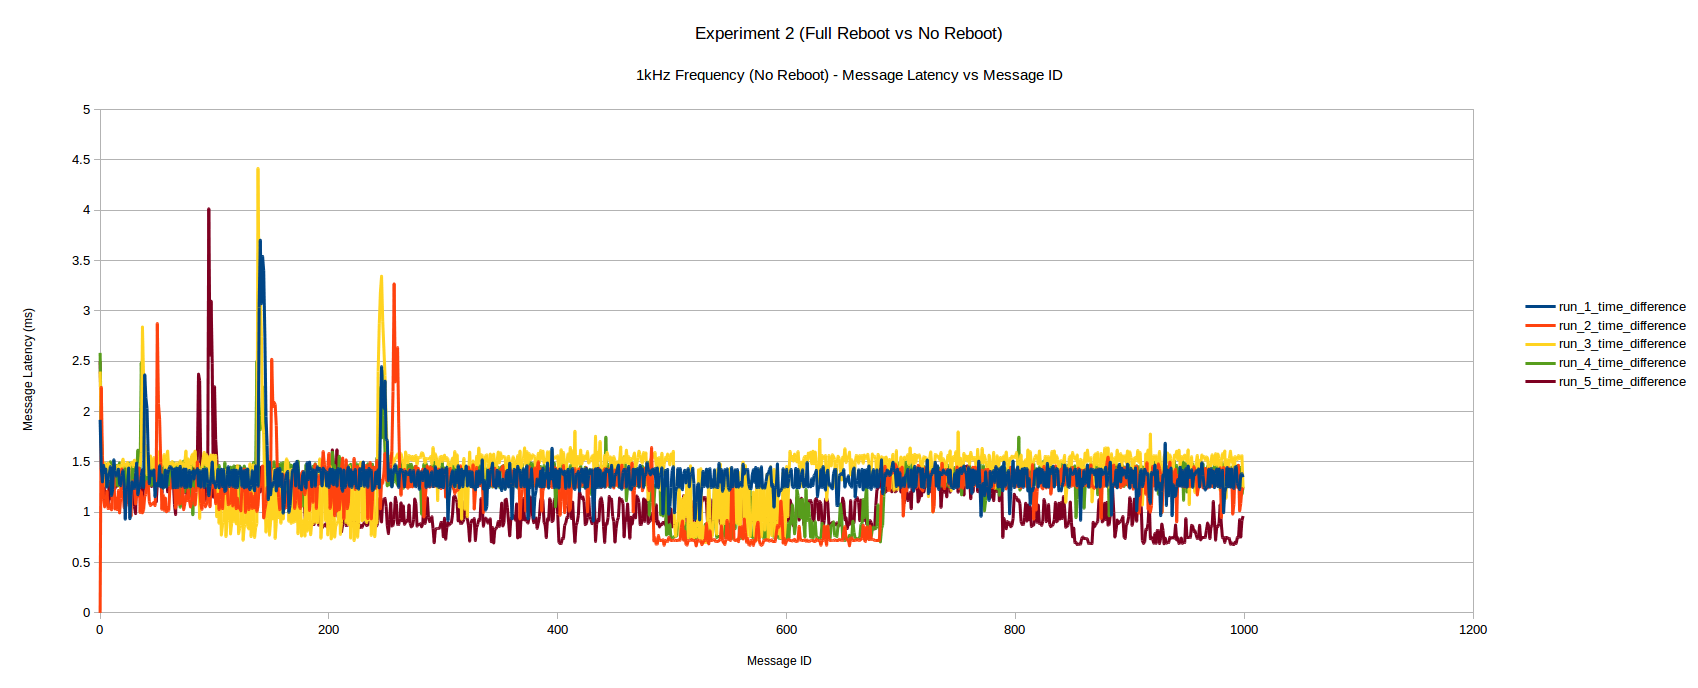
\includegraphics[width=\textwidth]{images/no-reboot-1khz.png}
\caption{Experiment 2 - No Reboot 1KHz Message Frequency}
\label{exp2-noreboot-1khz}
\end{figure}
Other graphs commented out for now.
\iffalse
\begin{figure}
\centering
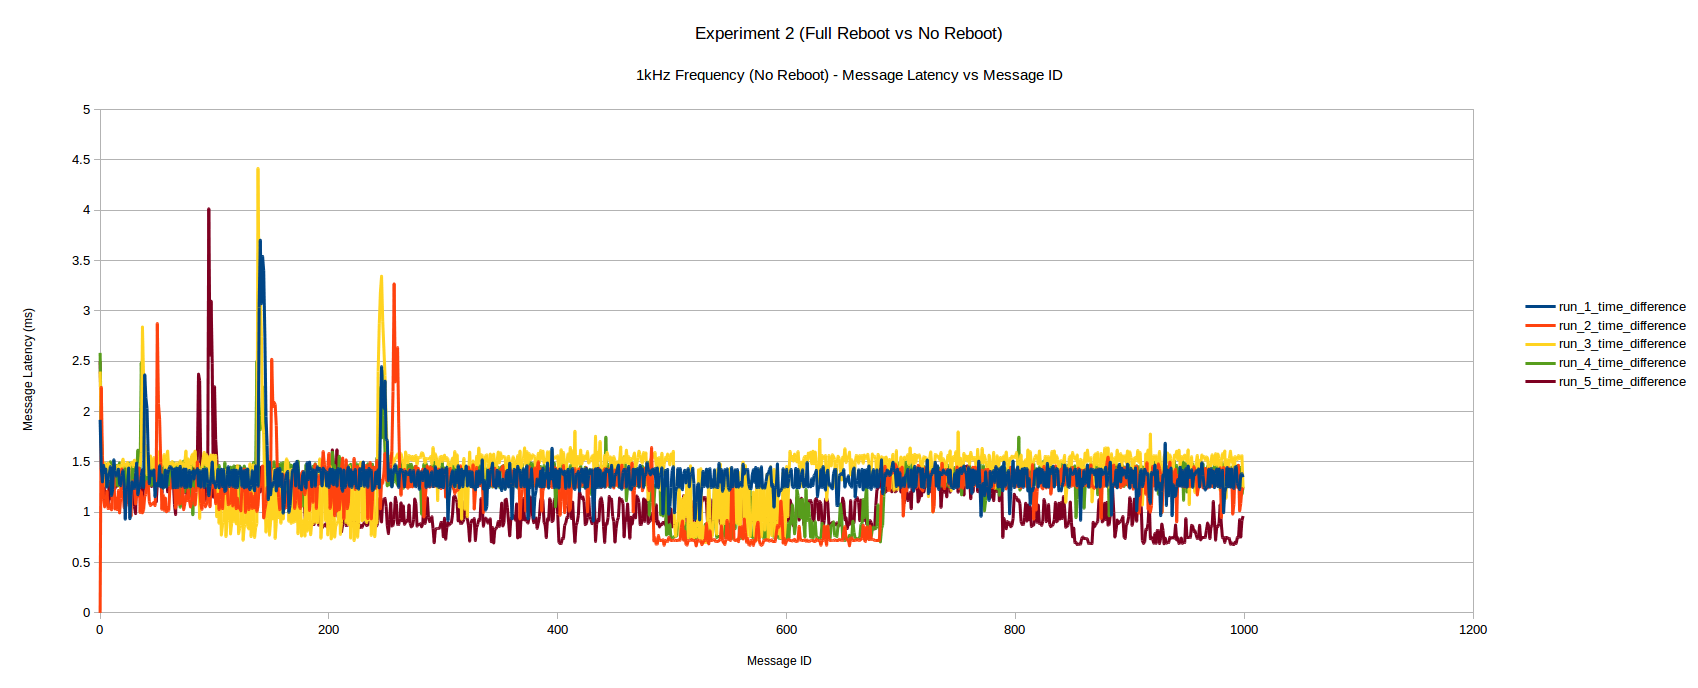
\includegraphics[width=\textwidth]{images/no-reboot-1khz.png}
\caption{Experiment 2 - No Reboot 1KHz Message Frequency}
\label{exp2-fullreboot-1khz}
\end{figure}

\begin{figure}
\centering
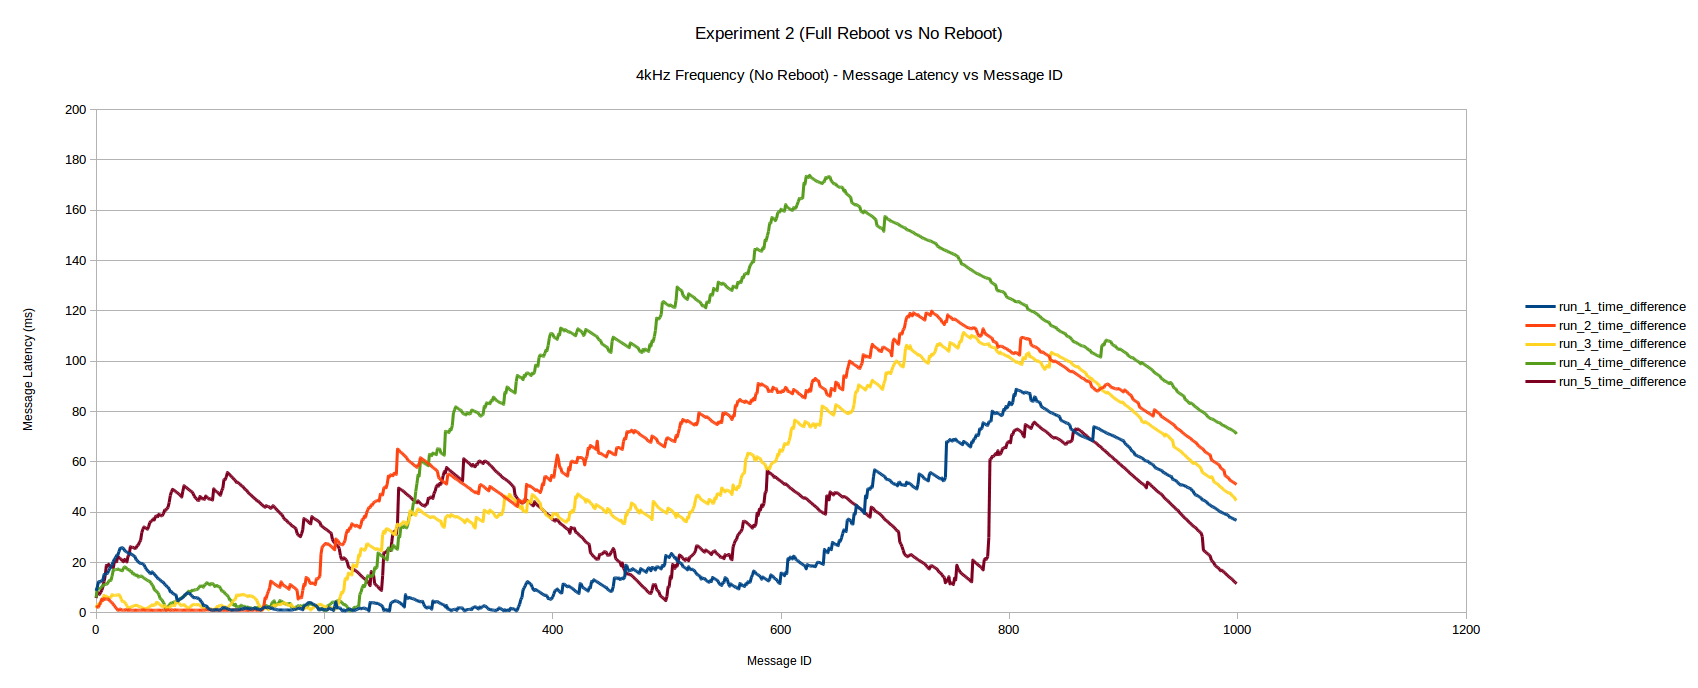
\includegraphics[width=\textwidth]{images/no-reboot-4khz.png}
\caption{Experiment 2 - No Reboot 4KHz Message Frequency}
\label{exp2-noreboot-4khz}
\end{figure}

\begin{figure}
\centering
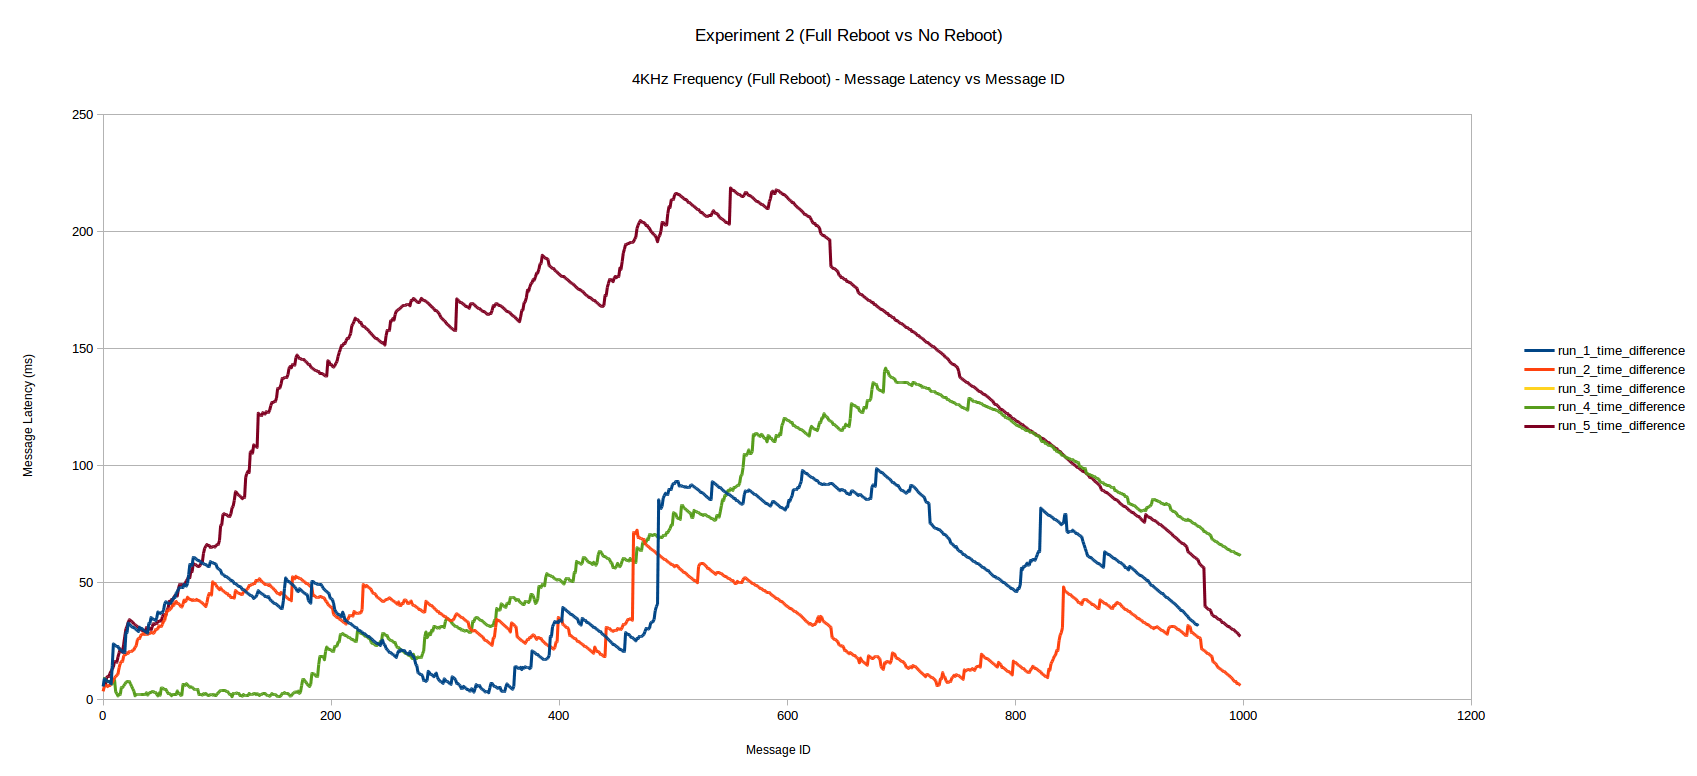
\includegraphics[width=\textwidth]{images/full-reboot-4khz.png}
\caption{Experiment 2 - Full Reboot 4KHz Message Frequency}
\label{exp2-fullreboot-4khz}
\end{figure}

\begin{figure}
\centering
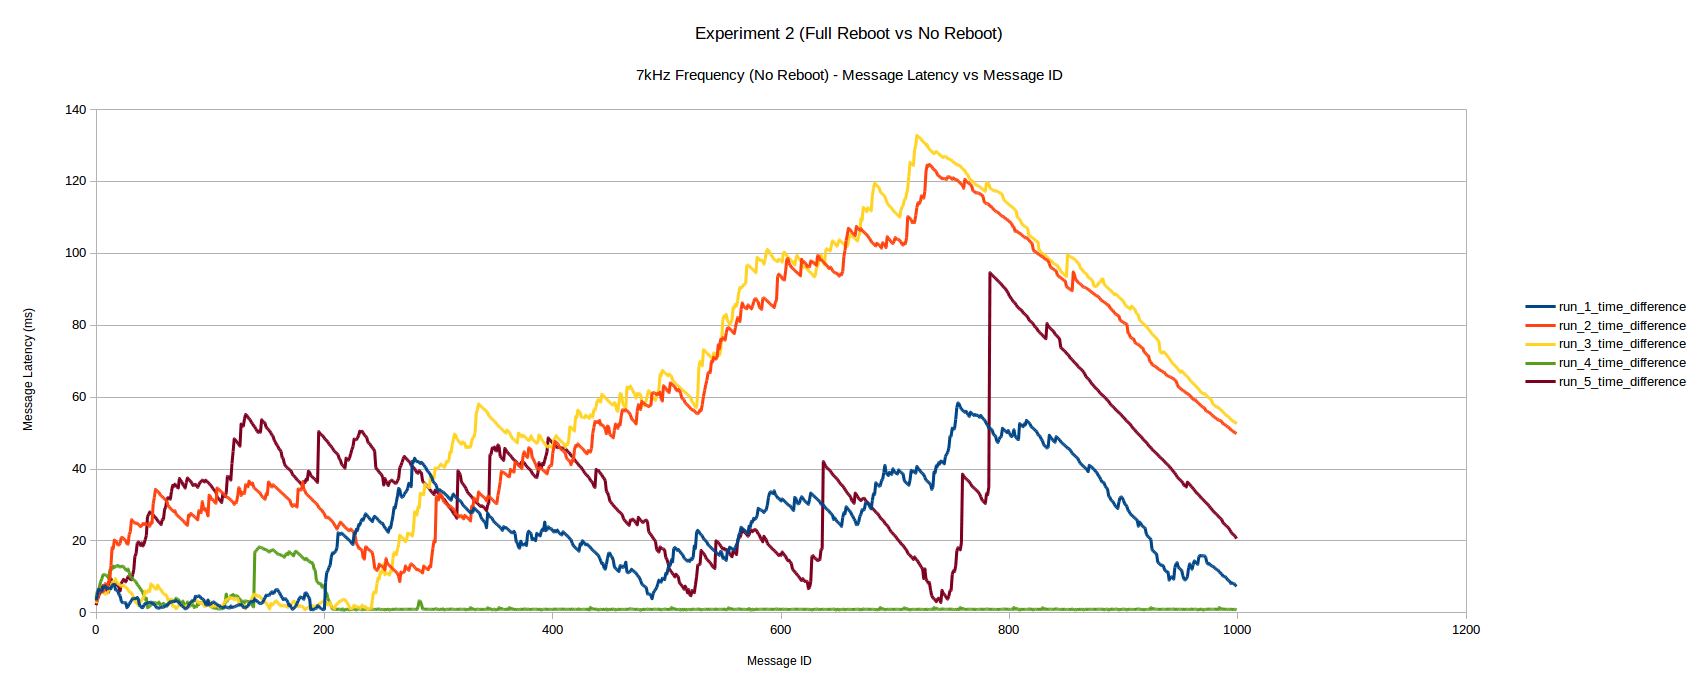
\includegraphics[width=\textwidth]{images/no-reboot-7khz.png}
\caption{Experiment 2 - No Reboot 7KHz Message Frequency}
\label{exp2-noreboot-7khz}
\end{figure}

\begin{figure}
\centering
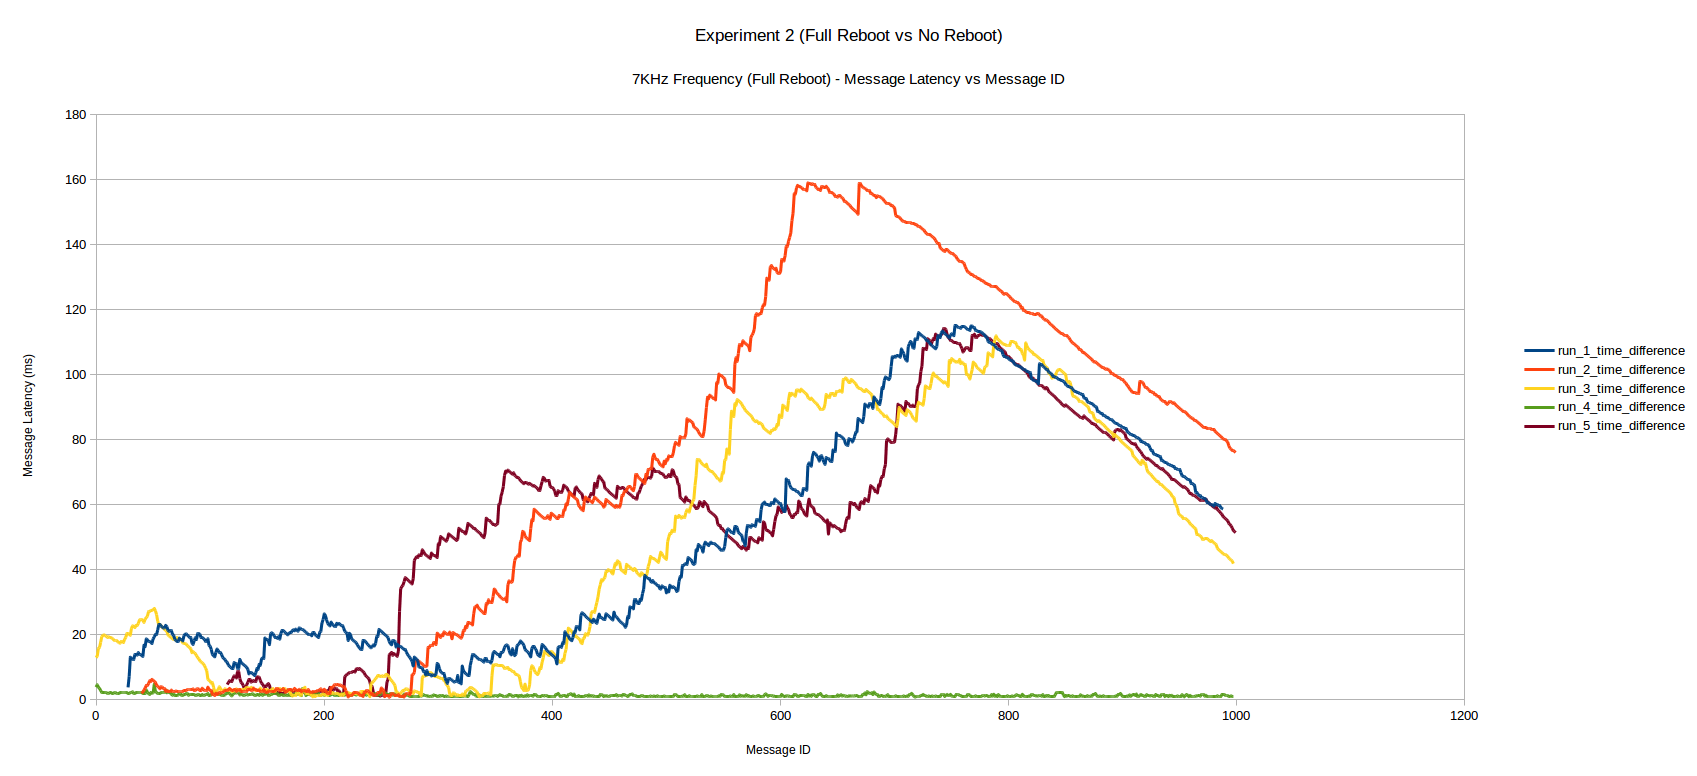
\includegraphics[width=\textwidth]{images/full-reboot-7khz.png}
\caption{Experiment 2 - Full Reboot 7KHz Message Frequency}
\label{exp2-fullreboot-7khz}
\end{figure}

\begin{figure}
\centering
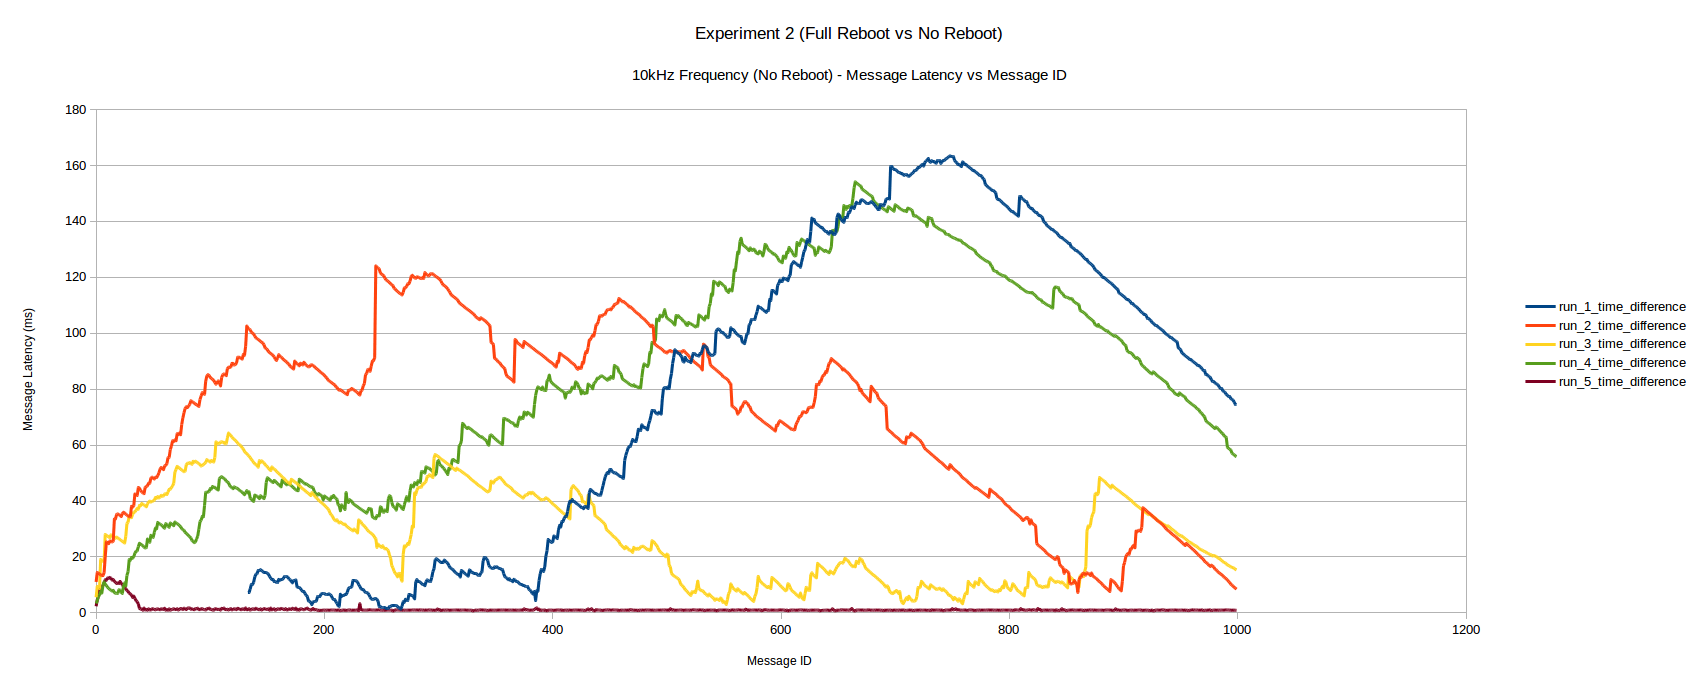
\includegraphics[width=\textwidth]{images/no-reboot-10khz.png}
\caption{Experiment 2 - No Reboot 10KHz Message Frequency}
\label{exp2-noreboot-10khz}
\end{figure}

\begin{figure}
\centering
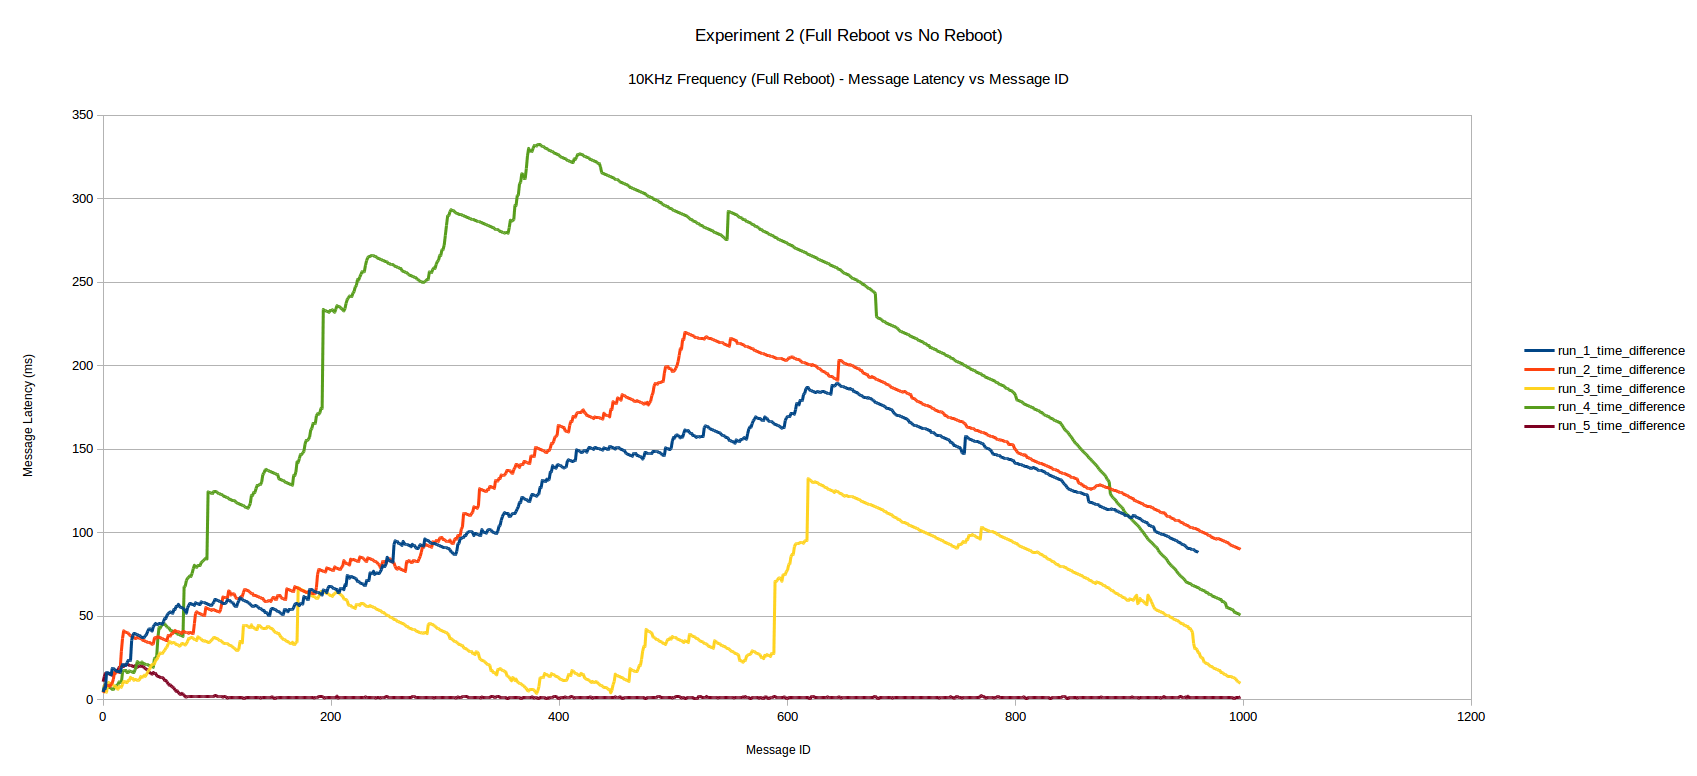
\includegraphics[width=\textwidth]{images/full-reboot-10khz.png}
\caption{Experiment 2 - Full Reboot 10KHz Message Frequency}
\label{exp2-fullreboot-10khz}
\end{figure}
\fi

\end{appendices}

%%%%%%%%%%%%%%%%%%%%
%   BIBLIOGRAPHY   %
%%%%%%%%%%%%%%%%%%%%

\bibliographystyle{plain}
\bibliography{bib}

\end{document}
